\documentclass[10pt]{beamer}

\usetheme[progressbar=frametitle]{metropolis}

\usepackage{booktabs}
\usepackage[scale=2]{ccicons}

\usepackage{pgfplots}
\usepgfplotslibrary{dateplot}

\usepackage{xspace}
\newcommand{\themename}{\textbf{\textsc{metropolis}}\xspace}
\usepackage{listings}
\title{Google Cloud Messaging}
\subtitle{Seminar}
\date{\today}
\author{Kevin Joseph}
\institute{College of Engineering, Trivandrum}
\begin{document}
\nocite{*}
\maketitle

\begin{frame}{Table of contents}
  \setbeamertemplate{section in toc}[sections numbered]
  \tableofcontents[hideallsubsections]
\end{frame}

\section{Introduction to Cloud}

\begin{frame}[fragile]{Cloud Computing}

  Cloud computing is a general term for the delivery of hosted services over the Internet. 

  Cloud computing enables companies to consume computer resources as a utility -- just like electricity -- rather than having to build and maintain computing infrastructures in-house. 
\end{frame}
\begin{frame}[fragile]{Types of Cloud Services}
  \begin{itemize}
		\item Software As A Service (SAAS)
		\item Platform As A Service (PAAS)
		\item Infrastructure As A Service (IAAS)
	\end{itemize}
\end{frame}

\section{Communication Between Cloud and Device}

\begin{frame}{Types of Communication}
	\begin{itemize}
		\item \textbf{Pulling}: The request for the transmission of information is initiated by the receiver or client. 
		\item \textbf{Pushing}: The request for a given transaction is initiated by the publisher or central server.
	\end{itemize}
\end{frame}

\section{Push Technology}

\begin{frame}[fragile]{Push}
      Push services are often based on information preferences expressed in advance. This is called a \textbf{publish/subscribe} model. A client "subscribes" to various information "channels" provided by a server; whenever new content is available on one of those channels, the server pushes that information out to the client.\\
      \vspace{5mm}\textbf{General Usage:} Synchronous Conferencing, instant messaging, email, etc
\end{frame}

\begin{frame}{Hosted Push Services}
Push notification services are available from several providers which support automated push notification campaigns:
  \begin{itemize}
    \item Apple Push Notification Service
    \item Google Cloud Messaging
    %\item Xtremepush
  \end{itemize}
\end{frame}

\section{Cloud To Device Messaging (C2DM)}

\begin{frame}[fragile]{C2DM}
      \textbf{Features:}\\
      \begin{itemize}
      		\item When messages are received on the Android client, the
system will wake up the application via an Intent broad-
cast, and pass the message data
		\item Developers are encouraged to
send short messages, essentially notifying the mobile
application that updated information can be retrieved
from the server
		\item Maxi-
mum number of messages that can be sent is approxi-
mately 200,000 per day
	\end{itemize}

      \vspace{5mm}\textbf{Disadvantages:} 
      	\begin{itemize}
      		\item Certain features, such as sending messages to
multiple clients, is not supported.
		\item The development environment and API could be better.
		\item In certain cases
quite a big increase in response times for some requests was seen.
	\end{itemize}
\end{frame}
\section{Google Cloud Messaging}

\begin{frame}[fragile]{GCM}
      Google Cloud Messaging (GCM) is a free service that enables developers to send messages between servers and client apps. This includes downstream messages from servers to client apps, and upstream messages from client apps to servers.
\end{frame}
\begin{frame}[fragile]{Components}
      \begin{itemize}
	    \item GCM Connection Servers
	    \item Client App
	    \item App Server
  \end{itemize}
  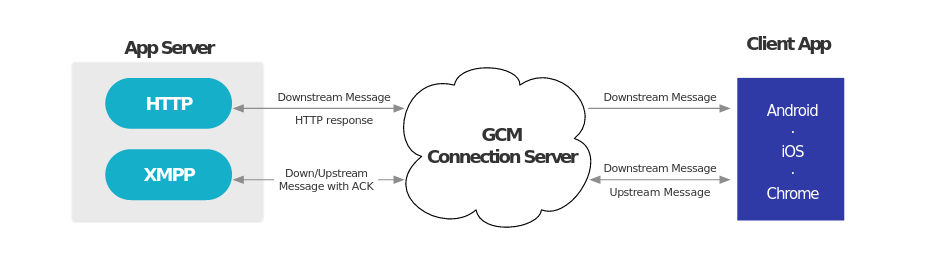
\includegraphics[width=\textwidth]{arch.png}
\end{frame}
\begin{frame}[fragile]{Credentials}
      \begin{itemize}
	    \item \textbf{Sender ID}: The sender ID is used in the registration process to identify an app server that is permitted to send messages to the client app.
	    \item \textbf{API Key}: An API key saved on the app server that gives the app server authorized access to Google services. In HTTP, the API key is included in the header of POST requests that send messages. In XMPP, the API key is used in the SASL PLAIN authentication request as a password to authenticate the connection
	    \item \textbf{Application ID}: The client app that is registering to receive messages.
	    \item \textbf{Registration Token}: An ID issued by the GCM connection servers to the client app that allows it to receive messages.
	\end{itemize}
\end{frame}
\begin{frame}[fragile]{Steps}
  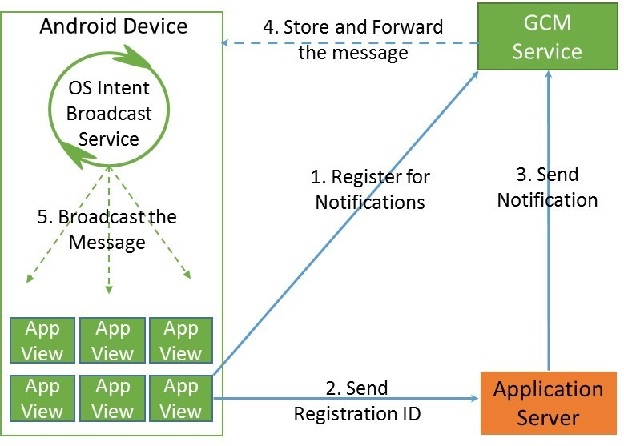
\includegraphics[width=\textwidth]{Steps.jpg}
\end{frame}
\begin{frame}[fragile]{Registering Client Apps}
  	\begin{itemize}
  		\item The client app must obtain a registration token using the Instance ID API.
  		\item Instance ID provides a unique ID per instance of your apps. 
  		\item Instance ID provides a simple API to generate security tokens that authorize third parties to access your app's server side managed resources.
  	\end{itemize}
\end{frame}
\begin{frame}[fragile]{Instance ID Lifecycle}
  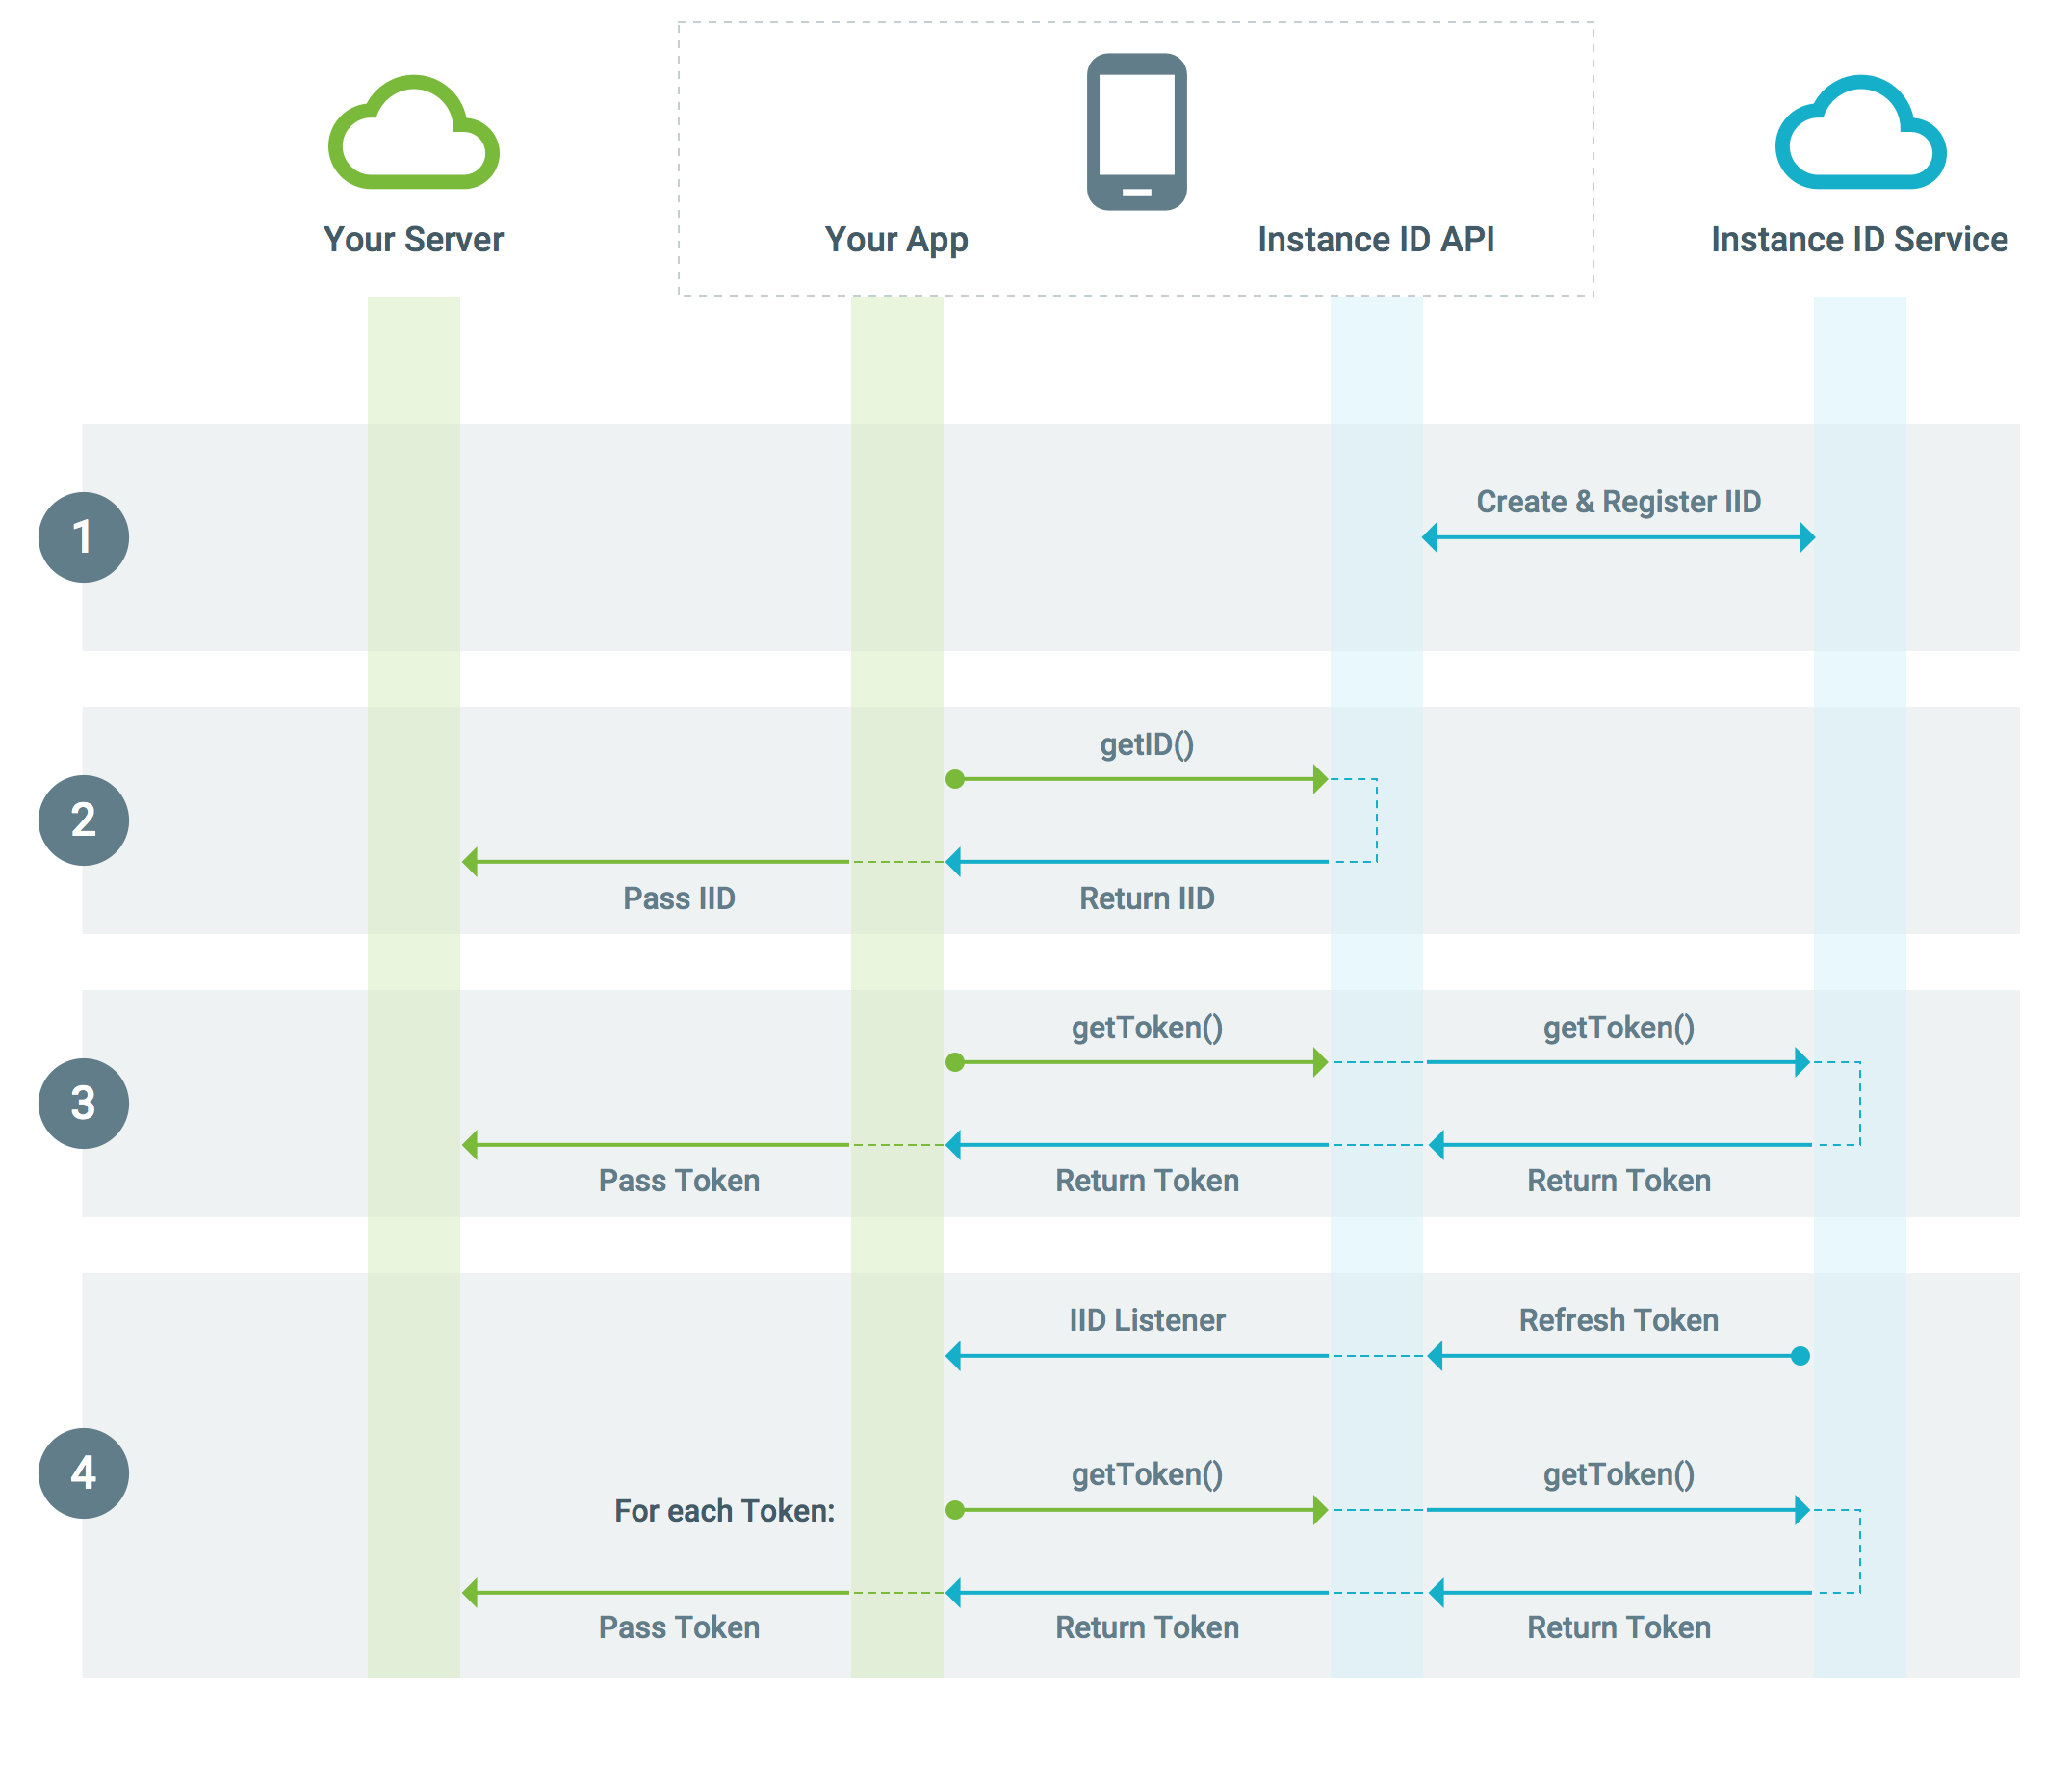
\includegraphics[width=\textwidth-10mm]{iid-lifecycle.png}
\end{frame}
\begin{frame}[fragile]{Android Implementation}
	\textbf{Get ID}
		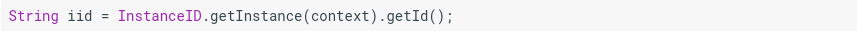
\includegraphics[width=\textwidth-10mm]{code1.png}\\
	\textbf{Generate Token}
		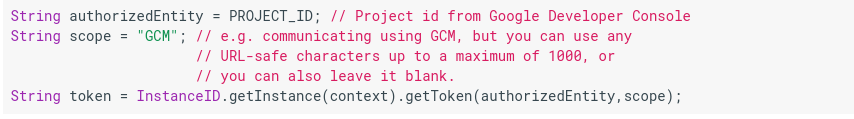
\includegraphics[width=\textwidth-10mm]{code2.png}\\
	\textbf{Refresh Token}
		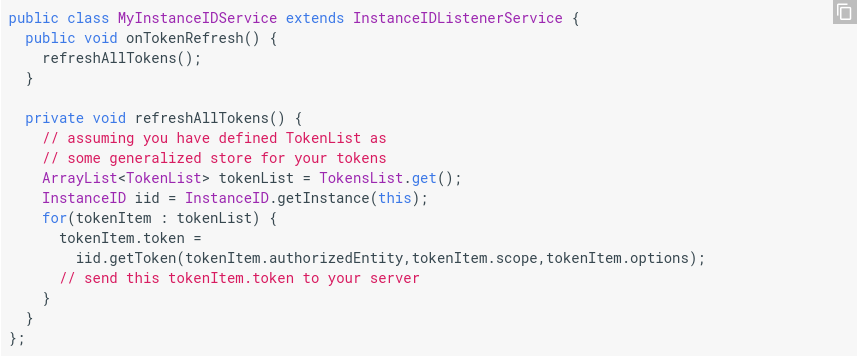
\includegraphics[width=\textwidth-10mm]{code3.png}
\end{frame}
\begin{frame}[fragile]{Uninstalled Client App Unregistration}
\begin{itemize}
  \item The app server sends a message to GCM connection server addressed to an uninstalled instance.
  \item The GCM connection server sends the message to the GCM client on the device.
  \item The GCM client on the device receives the message and detects that the client app has been uninstalled.
  \item The GCM client on the device informs the GCM connection server that the client app was uninstalled.
  \item The GCM connection server marks the registration token for deletion.
  \item The app server sends a message to GCM for the same instance.
  \item The GCM returns a NotRegistered error message to the app server.
  \item The app server should delete the registration token.
\end{itemize}
\end{frame}
\begin{frame}[fragile]{GCM Connection Servers}
The server side of GCM consists of two components:
\begin{itemize}
  \item Connection Servers 
  \item Application Servers
\end{itemize}
\end{frame}
\begin{frame}[fragile]{HTTP Server}
To send a message, the application server issues a POST request.A message request is made of 2 parts: HTTP header and HTTP body. The header must contain authorization and content-type.
\end{frame}
\begin{frame}[fragile]{Example}
\begin{lstlisting}
Content-Type:application/json
Authorization:key=AIzaSyZ-1u...0GBYzPu7Udno5aA

{
  "to" : "bk3RNwTe3H0:CI2k_HHwgIpoDKCIZvvDMExUdFQ3P1...",
  "data" : {
    ...
  },
}
\end{lstlisting}
\end{frame}
\begin{frame}[fragile]{Request Format}
\begin{itemize}
  \item \small\textbf{Send To Sync: } This is the smallest possible message
    \begin{lstlisting}
  { "to" : "bk3RNwTe3H0:CI2k_HHwgIpoDKCIZvvDMExUdFQ3P1..." }
    \end{lstlisting}
  \item \small\textbf{Message with payload — notification message: }
  \begin{lstlisting}
  { "notification": {
            "title": "Portugal vs. Denmark",
            "text": "5 to 1"
          },
    "to" : "bk3RNwTe3H0:CI2k_HHwgIpoDKCIZvvDMExUdFQ3P1..."
  }
    \end{lstlisting} 
  \item \small\textbf{Message with payload — Data message: }
  \begin{lstlisting}
  { "data": {
          "score": "5x1",
          "time": "15:10"
        },
    "to" : "bk3RNwTe3H0:CI2k_HHwgIpoDKCIZvvDMExUdFQ3P1..."
  }
    \end{lstlisting} 
\end{itemize}

\end{frame}
\begin{frame}[fragile]{XMPP Server}
The Google Cloud Messaging (GCM) Cloud Connection Server (CCS) is an XMPP endpoint that provides a persistent, asynchronous, bidirectional connection to Google servers. The connection can be used to send and receive messages between your server and your users' GCM-connected devices.
\end{frame}
\begin{frame}[fragile]{Request Format}
\begin{itemize}
  \item \small\textbf{Send To Sync: } This is the smallest possible message
    \begin{lstlisting}
  <message id="">
    <gcm xmlns="google:mobile:data">
    {
          "to":"REGISTRATION_ID",  
    }
    </gcm>
  </message>
    \end{lstlisting}
  
\end{itemize}
\end{frame}
\begin{frame}[fragile]{Request Format}
\begin{itemize}
  
  \item \small\textbf{Message with payload — notification message: }
  \begin{lstlisting}
  <message id="">
    <gcm xmlns="google:mobile:data">
    {
          "to":"REGISTRATION_ID",   
        "notification": {
            'title': 'Portugal',
            'text': 'test'
          },
          "time_to_live":"600"
  }
    </gcm>
  </message>
    \end{lstlisting} 
 
\end{itemize}
\end{frame}
\begin{frame}[fragile]{Request Format}
\begin{itemize}
  
 
  \item \small\textbf{Message with payload — Data message: }
  \begin{lstlisting}
  <message id="">
    <gcm xmlns="google:mobile:data">
    {
        "to":"REGISTRATION_ID",
          "message_id":"m-1366082849205"
          "data":
          {
            "hello":"world",
          }
          "time_to_live":"600",
          "delay_while_idle": true/false,
          "delivery_receipt_requested": true/false
    }
    </gcm>
  </message>
    \end{lstlisting} 
\end{itemize}
\end{frame}

\begin{frame}[fragile]{Performance Analysis}
\begin{itemize}
\item In GCM, push notifications to the same device are throttled using token bucket scheme.
\item The bucket holds 20 tokens and is replenished at a rate of once every 180 seconds.
\item The bucket appears to be completely replenished (randomly) every 0 to 90 minutes. 
\item When the bucket is out of tokens, push notifications are dropped instead of queued.
\end{itemize}
\end{frame}
\begin{frame}[fragile]{Performance Analysis}
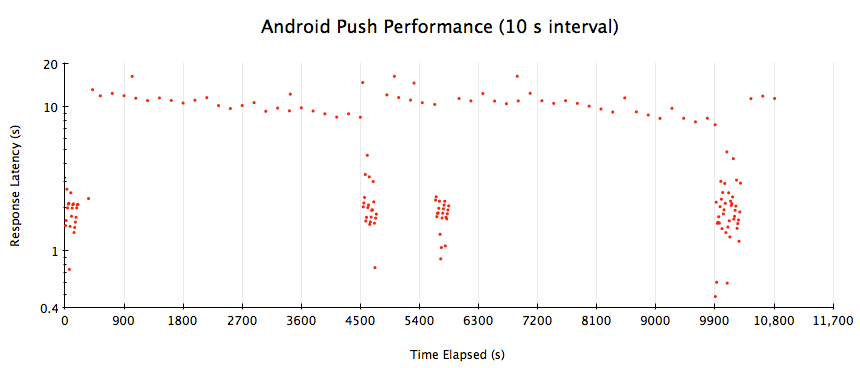
\includegraphics[width=\textwidth-10mm]{../report/images/graph1.png}
\end{frame}
\begin{frame}[fragile]{Performance Analysis}
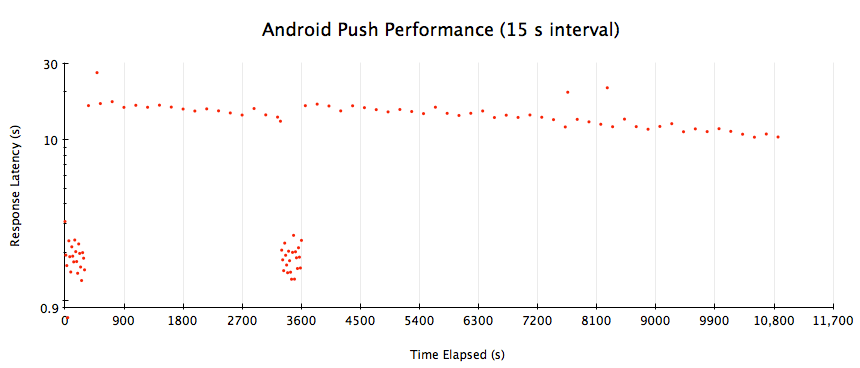
\includegraphics[width=\textwidth-10mm]{../report/images/graph2.png}
\end{frame}
\begin{frame}[fragile]{Performance Analysis}
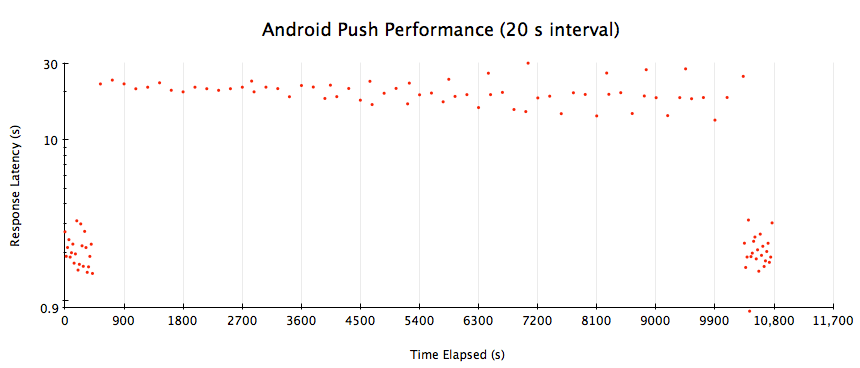
\includegraphics[width=\textwidth-10mm]{../report/images/graph3.png}
\end{frame}
\section{Firebase Cloud Messaging(FCM)}
\begin{frame}[fragile]{FCM architecture}
\begin{figure}[!htb]
\centering
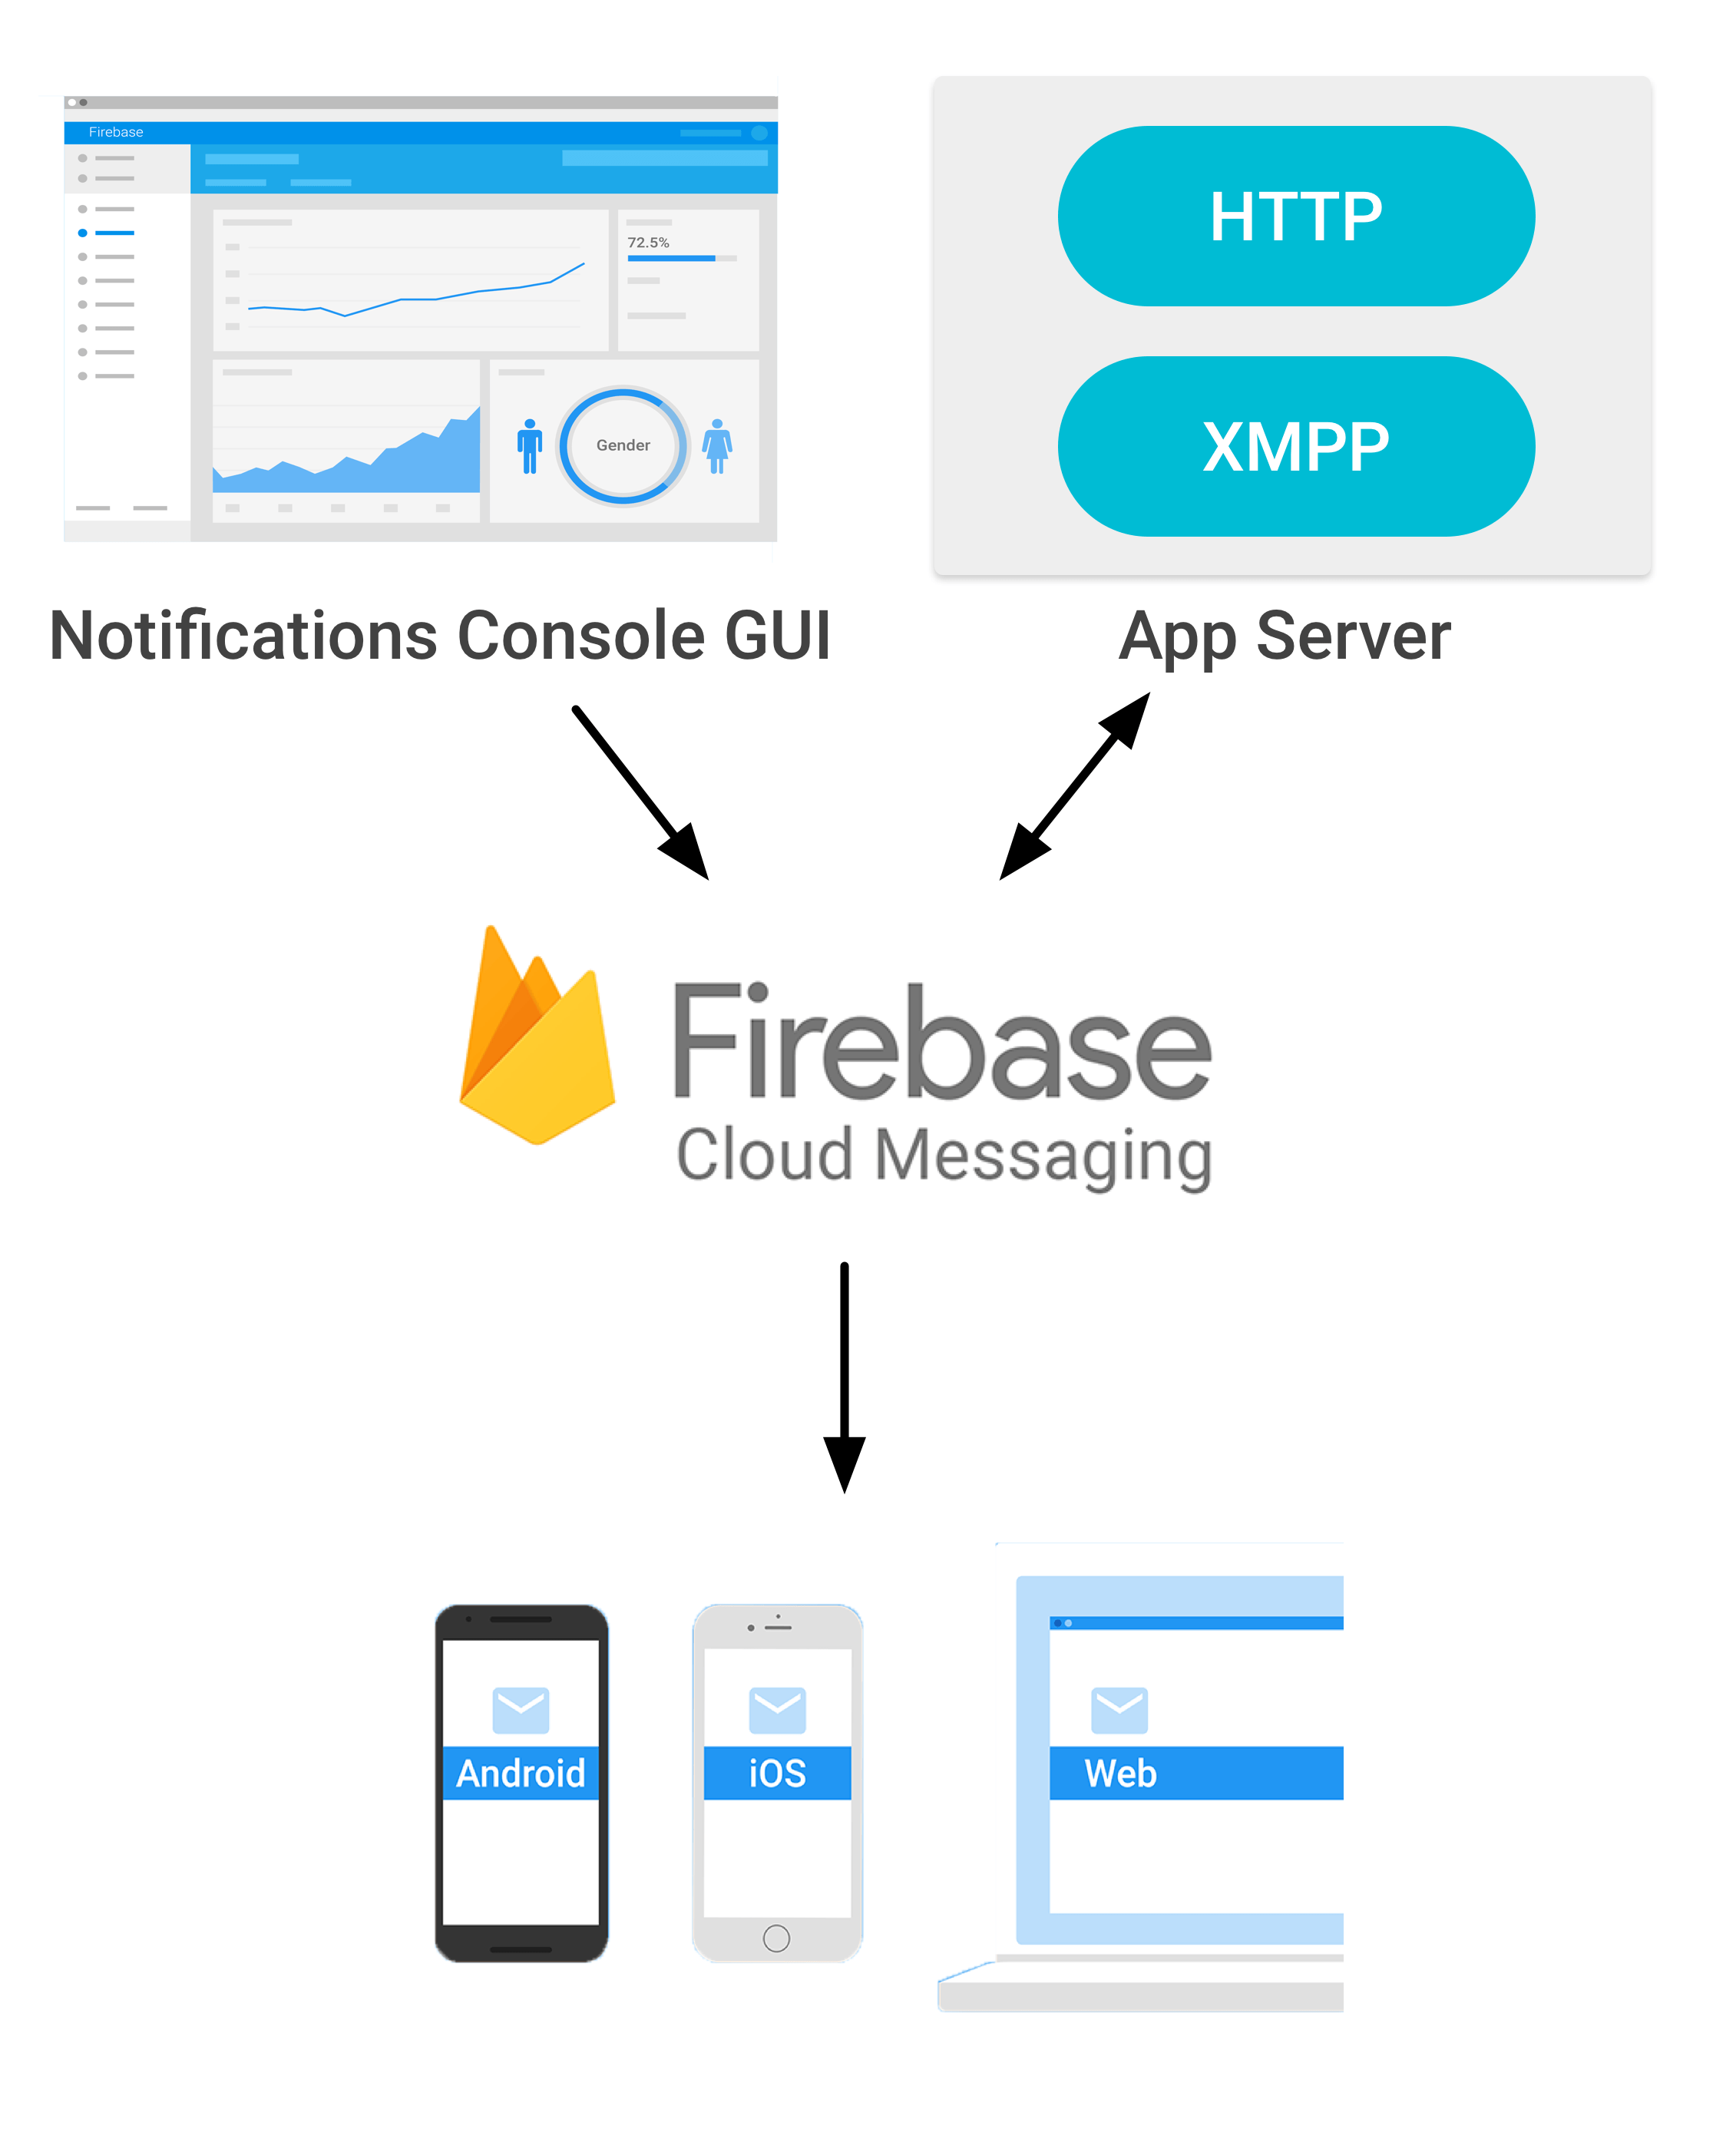
\includegraphics[width=5cm]{../report/images/fcm.png}
\end{figure}
\end{frame}
\begin{frame}[fragile]{FCM}
\begin{itemize}
\item Firebase Cloud Platform inherits GCM’s core infrastructure but simplifies the client development. Developers no longer needs to write their own registration or subscription retry logic. FCM includes a web console called Firebase Notifications which allows users to send notifications without an App server.
\item Firebase covers all that mobile developers need to build, maintain and scale a mobile app on all platforms (even on iOS): from Storage and databases to innovative tools like Remote Config and Test Lab.
\item Firebase also presents some performance improvements, it has an average response latency on 250ms and  95\% delivery rate which is a huge improvement when compared to 10s and 40\% on GCM.
\end{itemize}
\end{frame}
\section{Conclusion}
\begin{frame}[standout]
  Questions?
\end{frame}
\begin{frame}[allowframebreaks]{References}

  \bibliography{../common/seminar}
  \bibliographystyle{abbrv}

\end{frame}

\end{document}
